%%%% ijcai23.tex

\typeout{IJCAI--23 Instructions for Authors}

% These are the instructions for authors for IJCAI-23.

\documentclass{article}
\pdfpagewidth=8.5in
\pdfpageheight=11in

% The file ijcai23.sty is a copy from ijcai22.sty
% The file ijcai22.sty is NOT the same as previous years'
\usepackage{ijcai23}

% Use the postscript times font!
\usepackage{times}
\usepackage{soul}
\usepackage{url}
\usepackage[hidelinks]{hyperref}
\usepackage[utf8]{inputenc}
\usepackage[small]{caption}
\usepackage{graphicx}
\usepackage{amsmath}
\usepackage{amsthm}
\usepackage{booktabs}
\usepackage{algorithm}
\usepackage{algorithmic}
\usepackage[switch]{lineno}

% Comment out this line in the camera-ready submission
\linenumbers

\urlstyle{same}

% the following package is optional:
%\usepackage{latexsym}

% See https://www.overleaf.com/learn/latex/theorems_and_proofs
% for a nice explanation of how to define new theorems, but keep
% in mind that the amsthm package is already included in this
% template and that you must *not* alter the styling.
\newtheorem{example}{Example}
\newtheorem{theorem}{Theorem}

% Following comment is from ijcai97-submit.tex:
% The preparation of these files was supported by Schlumberger Palo Alto
% Research, AT\&T Bell Laboratories, and Morgan Kaufmann Publishers.
% Shirley Jowell, of Morgan Kaufmann Publishers, and Peter F.
% Patel-Schneider, of AT\&T Bell Laboratories collaborated on their
% preparation.

% These instructions can be modified and used in other conferences as long
% as credit to the authors and supporting agencies is retained, this notice
% is not changed, and further modification or reuse is not restricted.
% Neither Shirley Jowell nor Peter F. Patel-Schneider can be listed as
% contacts for providing assistance without their prior permission.

% To use for other conferences, change references to files and the
% conference appropriate and use other authors, contacts, publishers, and
% organizations.
% Also change the deadline and address for returning papers and the length and
% page charge instructions.
% Put where the files are available in the appropriate places.


% PDF Info Is REQUIRED.
% Please **do not** include Title and Author information
\pdfinfo{
/TemplateVersion (IJCAI.2023.0)
}

\title{How to boost a traditional indirect method for Monocular Visual Odometry
via deep neural networks}


% Single author syntax
\author{
    Kirill Brodt\\
    \affiliations
    \emails
    cyrill.brodt@gmail.com
}

% Multiple author syntax (remove the single-author syntax above and the \iffalse ... \fi here)
\iffalse
\author{
First Author$^1$
\and
Second Author$^2$\and
Third Author$^{2,3}$\And
Fourth Author$^4$
\affiliations
$^1$First Affiliation\\
$^2$Second Affiliation\\
$^3$Third Affiliation\\
$^4$Fourth Affiliation
\emails
\{first, second\}@example.com,
third@other.example.com,
fourth@example.com
}
\fi

\begin{document}

\maketitle

\begin{abstract}
    We present a simple improvement of traditional indirect method for
    Monocular Visual Odometry replacing classical feature detectors and feature
    matchers with deep neural network models. These models have good
    generalization performance without finetuning on specific task.
\end{abstract}

\section{Introduction}

Visual Odometry (VO) is the process by which the body ego-motion is inferred by
analyzing images captured while in motion. Scaramuzza and
Fraundorfer~\shortcite{scaramuzza2011vop1} present a general overview of the VO
pipeline as in the Figure~\ref{fig:vo_pipeline}. We follow the similar pipeline
except that we introduce deep neural networks for feature detection and feature
matching.

\begin{figure}
    \centering
    \includegraphics[width=1.0\linewidth]{./assets/pipeline.png}
    \caption{Visual Odometry pipeline \protect\cite{scaramuzza2011vop1}}
    \label{fig:vo_pipeline}
\end{figure}

\section{Methodology}

We observe that classical approaches based on ORB (or others) detectors and
FLANN (or others) matchers fail on this task. So, we focus our analisys on
feature detection and feature matching steps. We replace feature detection and
matching models with state-of-the-art dense feature matching deep neural
network model RoMa \cite{edstedt2023roma}. We further refine this matching with
another deep neural network model DeDoDe descriptor \cite{edstedt2023dedode}.
We use publicity available pretrained weights for mentioned models. Our method
doesn't require any retraining and has good generalization on new tasks. Though
one may improve the performance by finetunning the models to the specific task.

\section{Experiments}

We first rotate two consecutive frames and crop the bottom part of the image
with the static part of the car to remove the noisy feature detections. Then,
we resize the images to $W\times{}H=1344\times{}1712$ resolution and feed them
to RoMa model with default parameters to detect and match features. Finally, we
refine the matching using DeDoDe descriptor model. We show the example of RoMa
model's matching for two consecutive frames in Figure~\ref{fig:roma_kps}.

\begin{figure}
    \centering
    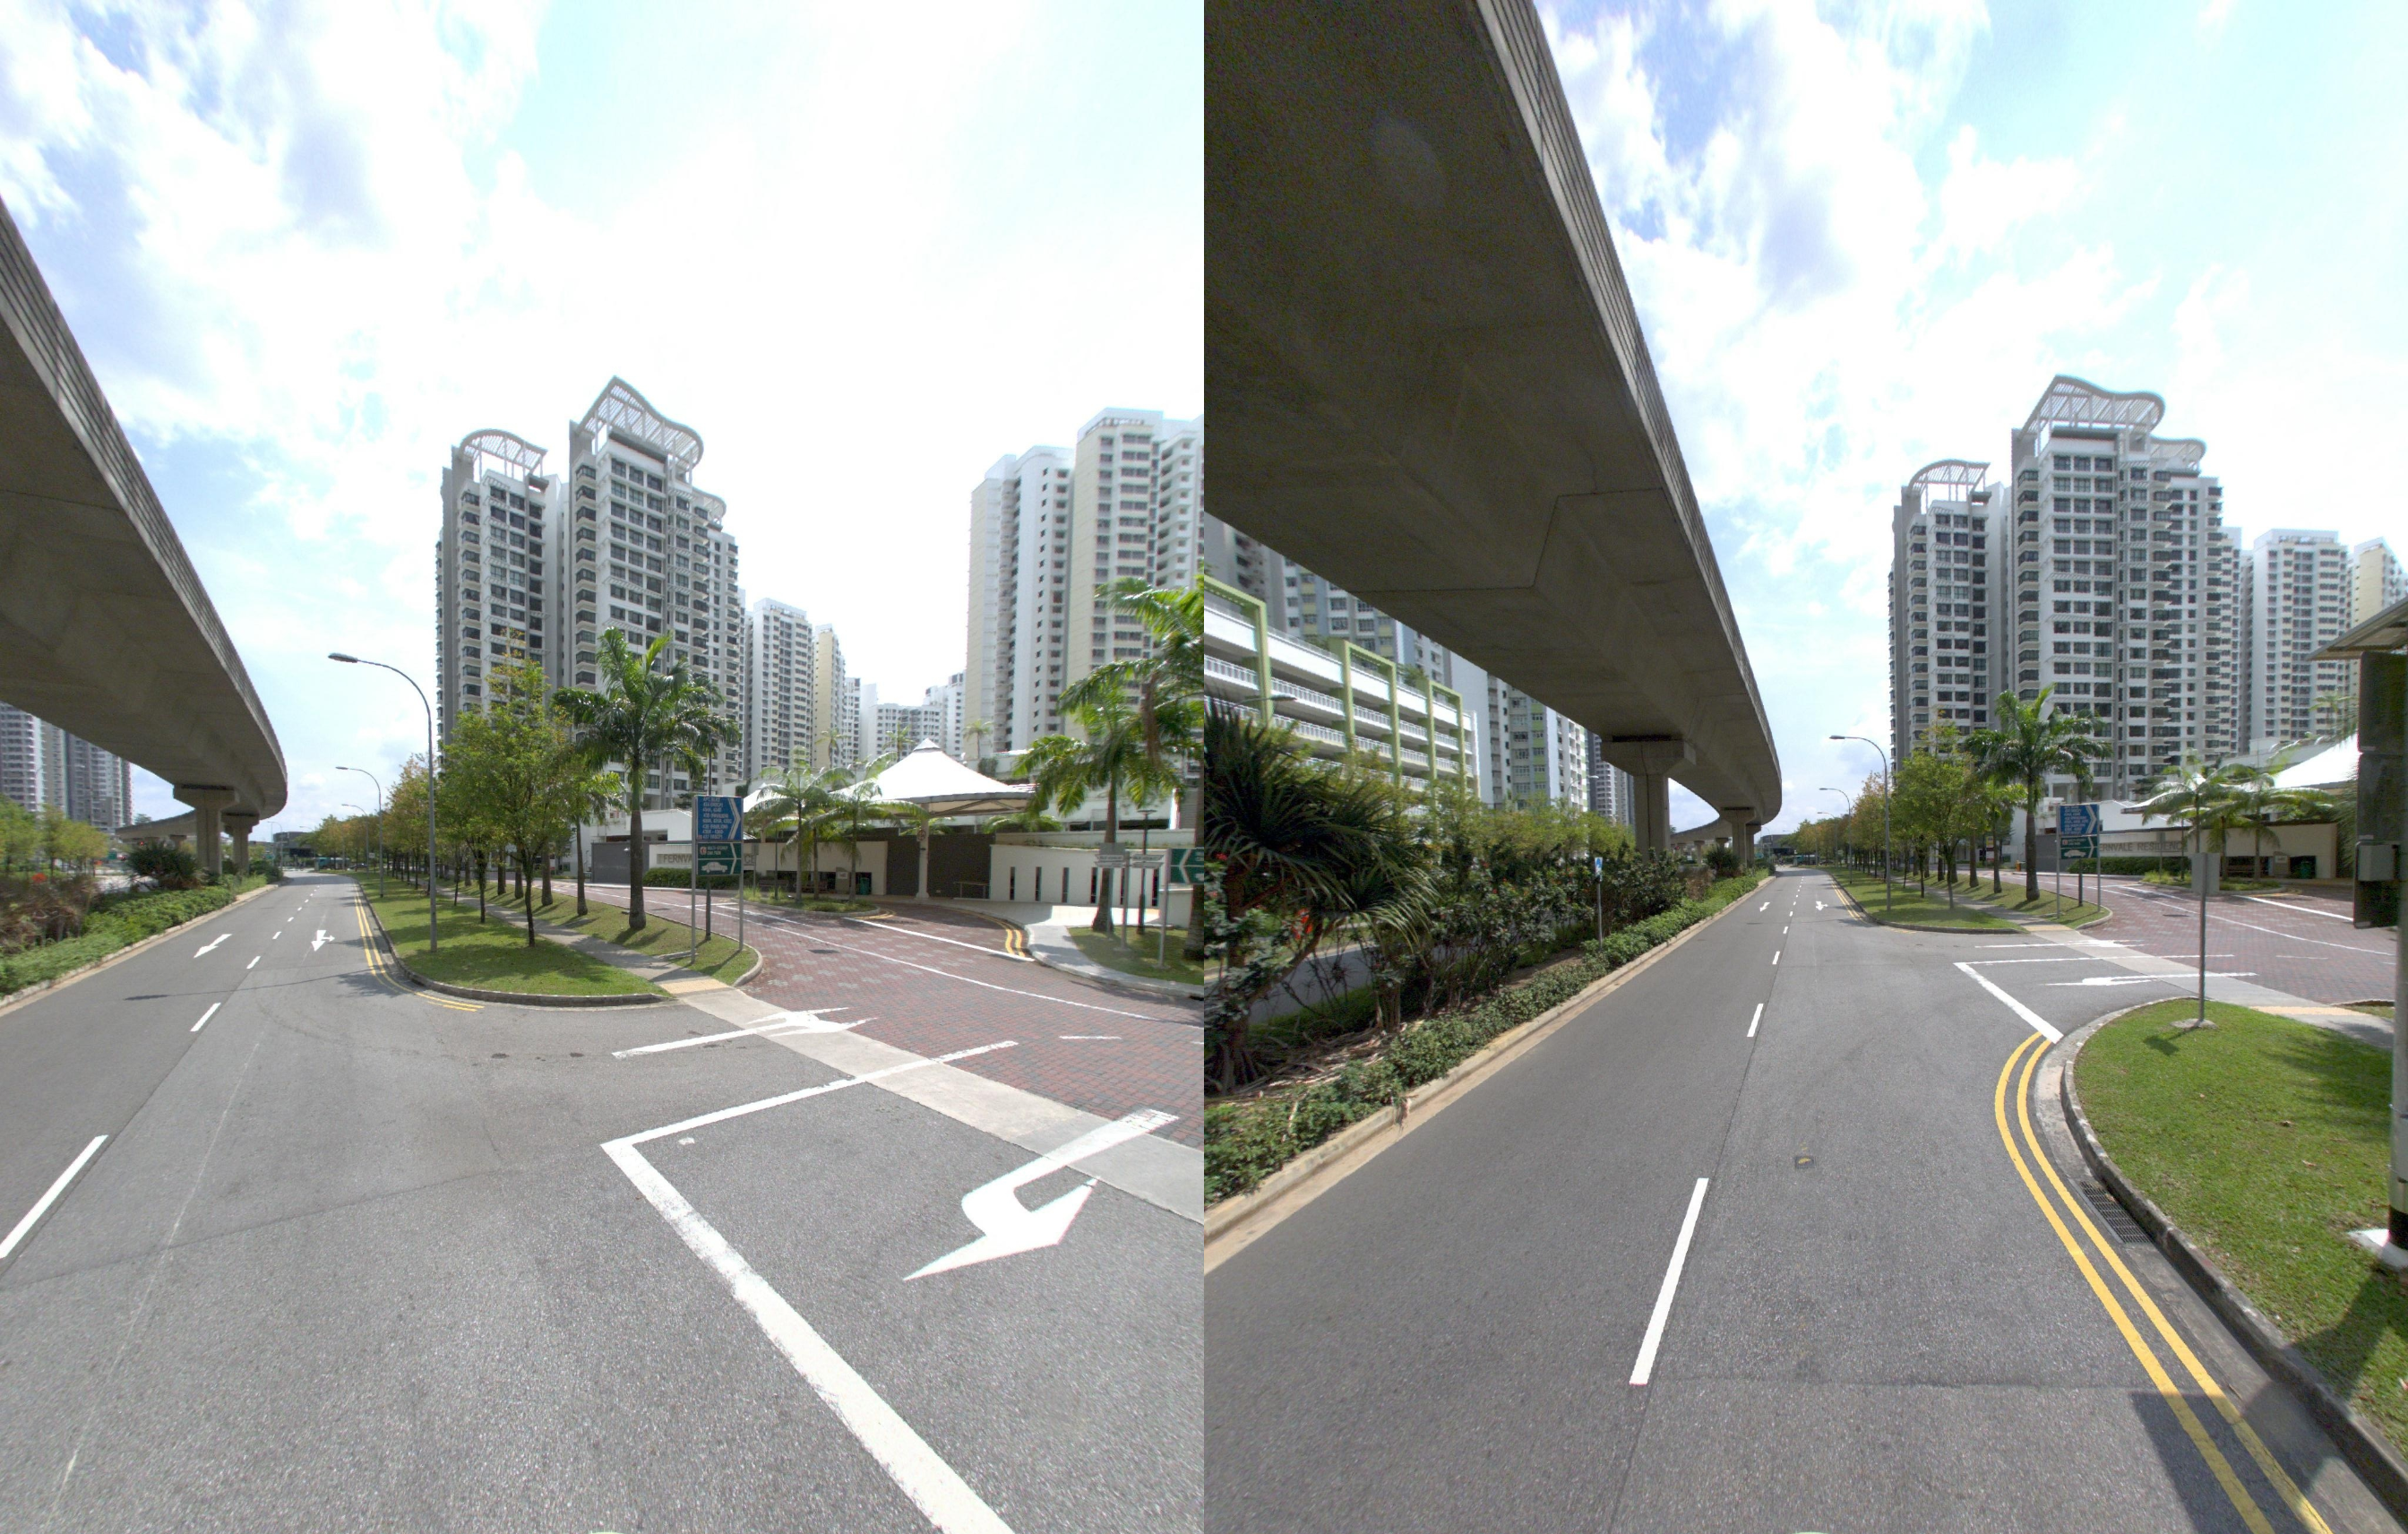
\includegraphics[width=1.0\linewidth]{./assets/inp.png}
    \includegraphics[width=1.0\linewidth]{./assets/roma.png}
    \caption{RoMa's dense matching (left \texttt{180426\_013227300\_Camera\_0},
    right \texttt{180426\_013228811\_Camera\_0})}
    \label{fig:roma_kps}
\end{figure}

After a set of features have been matched we use 2D-to-2D method to model the
motion between frames. We find the essential matrix with RANSAC algorithm with
confidence $0.99$ and threshold $1$ and recover the camera pose. To refine the
pose we further use local bundle adjustment implemented in
PyTorch~\cite{edstedt2023mba}. Note, that we use only two consecutive frames
and there is no way to determine the magnitude of translation between two
cameras. We use constant magnitude equal to $7.571103106907284$ calculated as a
mean of magnitudes from train trajectories.

\subsubsection{Evaluation metrics}

The performance metric is the rotational relative pose error of the estimated
camera poses:

\begin{equation}
    E_{rot}
    =\frac{1}{\mathcal{F}}
     \sum_{(i,j)\in\mathcal{F}}
     \angle
     \left[
         \left(\mathbf{\hat{p}_j} \ominus \mathbf{\hat{p}_i}\right)
         \ominus
         \left(\mathbf{p_j} \ominus \mathbf{p_i}\right)
     \right],
\end{equation}
where $\mathcal{F}$ refers to a set of frames belonging to a single trajectory
and $(i,j)$ denotes two adjacent frames within the sequence. $\mathbf{\hat{p}}$
and $\mathbf{p}$ are the estimated and ground true camera pose coordinates,
respectively, $\ominus$ denotes the inverse compositional operator and
$\angle[\cdot]$ represents the rotation angle.

\begin{table}
    \centering
    \begin{tabular}{lrrr}
        \toprule
        Trajectory & \multicolumn{2}{r}{Rotational Error} & Runtime (min) \\
        %& \multicolumn{1}{c}{Ours} & \multicolumn{1}{c}{Stationary} & \\
        & Ours & Stationary & \\
        \midrule
        1 (1398 frames) & 0.0433 & 0.1972 & 35 \\
        2 (1301 frames) & 0.0469 & 0.2026 & 33 \\
        3 (4914 frames) & 0.0144 & 0.0954 & 125 \\
        4 (2390 frames) & 0.0202 & 0.1037 & 61 \\
        \midrule
        5 (2218 frames) & 0.0382 & 0.2028 & 56 \\
        \bottomrule
    \end{tabular}
    \caption{Rotational relative pose error over different trajectories.}
    \label{tab:metric}
\end{table}

\subsubsection{Results}

We show the resulting metrics over five different trajectories in
Table~\ref{tab:metric}. We compare our method with the stationary camera model
(constant predictions) and see the 5x improvement on average. We also tried a
classical non-deep learning approach with ORB detector and FLANN matcher and
didn't manage to get better performance than the stationary camera. Therefore,
we don't show the metrics for the classical algorithms. We show the predicted
sub-trajectories for trajectory~1 in Figure~\ref{fig:traj1}.

\begin{figure}
    \centering
    \includegraphics[width=1.0\linewidth]{./assets/traj1_07.png} \\
    \bigskip
    \includegraphics[width=1.0\linewidth]{./assets/traj1_11.png}
    \caption{Examples of some predicted sub-trajectories of our method. Note,
    that here we use ground truth magnitudes of translation vectors between two
    cameras for improved presentation. The titles represent rotation error
    (RE).}
    \label{fig:traj1}
\end{figure}

\subsubsection{Performance}

We have implemented our method in Python using OpenCV and PyTorch libraries.
All the results presented in the report were computed with the default
parameters presented in the text and on the machine with single core of Intel®
Xeon® Gold 6148 CPU @ 2.40GHz, 4GM RAM and NVIDIA® Tesla® V100-SXM2 32GB. The
actual GPU VRAM usage is 16GB. The full pipeline performs 0.65fps or 1.5s per
frame.

%% The file named.bst is a bibliography style file for BibTeX 0.99c
\bibliographystyle{named}
\bibliography{ijcai23}

\end{document}
